\chapter{Results}
\label{chapter:Results}


\section{Using graph convolution in the way it's meant to be used gives poor results on molecular structures}

In the paper Chen et al.~\cite{Chen2019} at Tencent Lab, the authors modify a well performing GCNN architecture for quantum chemistry invented by Gilmer et al.~\cite{Gilmer2017}. The authors expand this model by using both, categorical bond type and euclidean distance as edge features and observe considerably better performance. At first glance, the use of both kinds of features - which seems to be implied in the paper - looks like a plausible explanation for the success. However, a upon closer inspection, the reasoning does not add up. Bond types almost completely determine the euclidean distance. E.g. ever carbon-carbon single bond has a distance of []Å, every carbon-oxygen double bond is []Å long, etc. [CITATON]. (The same applies to the reverse: knowing the distance between two atoms as well as the atom types allows to deduce the type of covalent bond or lack thereof.) Therefore no additional information is added by including the euclidean distance as a feature. Inspection of the implementation reveals anther possible reason for the good performance of the Tencent Lab-paper is quickly identified: Not only is the euclidean distance added as a feature to existing edges, every atom is connected to every other atom in the molecule with the euclidean distance being the only not-null feature~\footnote{\url{https://github.com/tencent-alchemy/Alchemy}}. Thus, the structure of the graph is changed dramatically form the graph of covalent bonds to complete graph where every node is connected to every other node. The complete graph is a special case of graph and is rather untypical because in most applications, the presence or absence of an edge between two nodes is the most important kind of information. Simply connecting all nodes with each other seems to diminish this information (although in this case, the euclidean distance allows to distinguish between important and less important edges). With these considerations it is surprising but very interesting that the approach of Tencent Labs works so well.

In preparation for this thesis, I participated in the Tencent-Alchemy competition~\footnote{\url{https://alchemy.tencent.com}} using approach described above a baseline architecture. Despite many experiments, I achieved the best results simply fine-tuning Tencent Labs model and finished 26th out of 53 participants. The fact that half the participants did not beat the baseline published in the official competition paper, shows that the approach is indeed quite effective an warrants a closer examination why the peculiar approach of using complete graphs works quite well.

%As discussed in the introduction, a central concept of graph convolution (and regular convolution as well), is to compute a representation of a local neighborhood. In the case of graphs, a local neighborhood is a node and its neighbor nodes while on images, it is a small patch of pixels, such as 3x3 or 5x5.


As explained in the introduction, we can define the neighborhood of a node as all other nodes within a certain distance threshold. We refer to this threshold as neighborhood radius.

Therefore, the first experiment, we compare the learning curves of graphs when defining the neighborhood with different thresholds. First of all, covalent bonds are always represented as edges in the graph. Then, for increasing radii, edges to all non-covalently bonded atoms within the radius are added to the graph. A neighborhood radius of zero thus means that no additional edges are added to the graph - the graph only has edges between covalently bonded atoms. At a radius of 1.5 Ångström (1Å = 10nm), an edge is added between any two non-covalently bonded atoms with a distance of at most 1.5Å. The same is done for 2Å, etc. For perspective, most covalent bonds in organic molecules have a distance of around 1Å [CITATION]. 1.5Å is very close for non-covalently bonded atoms such that only very few non-covalently bonded atoms - if any - will be within 1.5Å of an atom in an organic molecule. With a 2Å radius, every atom in the molecule will get some new neighbors due to this rule. With a 4Å radius, many atoms will be included in the neighborhood that have very little to no interaction with the central atom. At 5Å, for many small molecules, every atom is considered a neighbor of any other atom - applying this radius is therefore similar to connecting every atom with every other atom in the molecule. Finally, with an infinite radius, a complete graph is obtained.

\begin{figure}[H]
	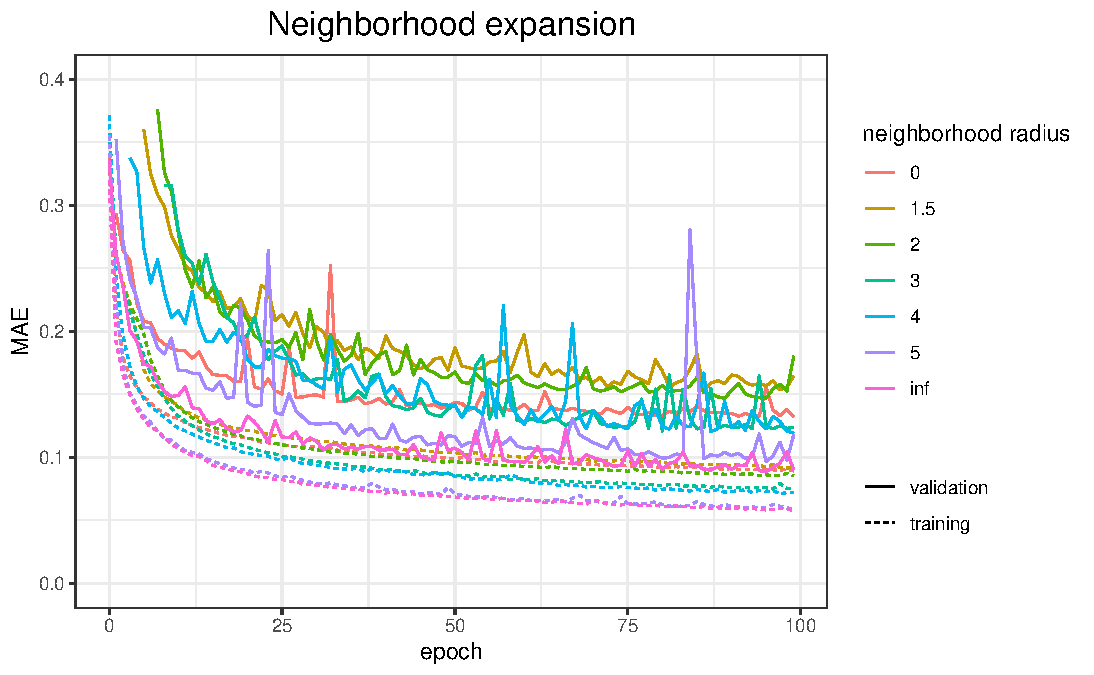
\includegraphics[width=\linewidth]{figures/tencent-mpnn-neighborhood-expansion}
	
	\caption{The learning curves with different neighborhood radii are show over the courses of 100 epochs. The color corresponds to the neighborhood radius, dotted lines the training errors and solid lines show validation errors. Note that for each radius, there is a training- and a validation-error curve. Each curve is an average of three learning curves with the same neighborhood radius. All curves were generated using a simple optimization scheme described in Section~\ref{sec:training}. Both, validation- and training-error could be lowered considerably by employing a more sophisticated optimization scheme. However, this would be at the expense of comparability between curves.[REFERENCE]}
	\label{fig:tencent-mpnn-neighborhood-expansion}
\end{figure}

As Figure~\ref{fig:tencent-mpnn-neighborhood-expansion} shows, the best performance is indeed achieved with the complete graph - connecting every atom with every other atom in the molecule with an edge. In general, the larger the neighborhood radius, the better the performance~\footnote{Exception: radius 0}. This result is in line with the suspicion that the real reason for the good performance of Tencent Lab's model is the addition of new edges rather than the addition of the euclidean distance feature.
The result is somewhat counterintuitive and in contrast with the principle of (graph-)convolution. As described in the introduction, in theory, graph convolutions update node-representation based on the local neighborhood of each node. Eventually, after $t$ layers, each node representation would contain indirect contributions from all other nodes with $t$ or less edges between. However, the results shown here show that the performance is best if the graph convolution considers all atoms at every layer. This contrast clearly shows that much remains to be discovered about the use of GCNN for molecules.

For small molecules and with considerable computational power at hand, one could simply accept this finding as it is and represent molecules as complete graphs. However, for larger molecules with hundreds of atoms, this would be computationally not feasible as the number of edges increased quadratically ($\frac{n(n - 1)}{2}$ edges for $n$ nodes). Therefore, further experiments will aim at finding an alternative way that captures the advantage of the complete graph-approach without the excessively high computational cost.


%Show that, for decreasing thresholds, performance decreases
%
%Emphasize that this is not really appreciated in the literature.
%Cite Alchemy paper and point out that the high-performing kaggle-teams all use fully connected graphs.
%Does no one notice?
%
%Repeat that the conv should be able to handle this because after several MP steps, the effective field of vision is the entire molecule - but it doesn't work well


\section{Manual feature engineering does not improve prediction accuracy.}

% compare raw vs. tencent features.
% after the point has been made, use only raw data

\section{Excluding hydrogen atoms from the molecule-graph speeds up training but reduces prediction accuracy}

Another possible preprocessing step is to disregard hydrogen atoms and instead add the number of hydrogen atoms bonded to a given heavy atom as a node feature. The rational behind this step is that the properties chemical properties of hydrogen atoms depend strongly on the heavy atom to which it is bound. While some information is lost during this step, the number of atoms in the molecule is reduced by an average factor of [CHECK value]. This modest reduction in the number of nodes leads to a very dramatic reduction in the number of edges. Naturally, this effect is most pronounced in complete graphs where the number of edges increases quadratically with the number of nodes ($\frac{n(n - 1)}{2}$ edges for $n$ nodes). While the average number of edges using complete graphs is [CHECK value] in the AlChemy dataset, this number drops to [CHECK value] after excluding hydrogen atoms.

The approach of not considering hydrogen atoms explicitly but only as features of heavy atoms is known as using \textit{implicit hydrogen atoms}. In short, it is a way of summarizing raw data which speeds up training considerably while loosing some information. Figure [] shows...

% probably: larger error
% => use explicit hydrogen atoms from now on


\section{Introducing a graph-state at every graph-conv layer improves results}



{\itshape
explain hypothesis:
lack of information of global environment. Maybe graph-level features needed at every conv?

Test this hypothesis:
add graph-state
show figure: now the effect is less pronounced because the global environment is accessible through the graph-state

Why this is important:
in larger graphs the option of using a fully connected graph is simply not there:
show computational complexity graph
}


\section{graph-conv layers with independent weights do not improve results}

{\itshape
	
OPTIONAL SECTION

It's reasonable to assume, that different layers need different feature extraction properties (low vs. high level features). In cv, the layers don't share weights.

However, in experiments, the weight-shared graph layers prove superior.
}

\section{relative position edge features improve results slightly}

{\itshape
 Show that relative position edge features slightly improve the results but not much
 
 explain that the problem is probably that they are not rotation-invariant
	
	
OPTIONAL PART:\\
review the results of the 3DGCN-paper and show that this doesn't work really well on the Alchemy data - probably for the same reason given above
}






